%% SHADE — IEEE conference paper draft.
%% Compile on Overleaf (recommended): New Project -> Upload -> select this paper/ folder,
%% set compiler to pdfLaTeX, main file = main.tex. Or locally: pdflatex; bibtex; pdflatex x2.
\documentclass[conference]{IEEEtran}
\IEEEoverridecommandlockouts
\usepackage{cite}
\usepackage{amsmath,amssymb,amsfonts}
\usepackage{graphicx}
\usepackage{booktabs}
\usepackage{url}

\begin{document}

\title{When Does Supervised NIDS Generalize to Unseen Attacks?\\
A Leave-One-Family-Out Study with Explainable Anomaly Backup}

\author{
\IEEEauthorblockN{Kanishk Sigar}
\IEEEauthorblockA{\textit{Dept. of CSE}\\
\textit{Graphic Era Hill University}\\
Dehradun, India\\
kanishksigar@gmail.com}
\and
\IEEEauthorblockN{Mohammad Wazid}
\IEEEauthorblockA{\textit{Dept. of CSE}\\
\textit{Graphic Era (Deemed to be Univ.)}\\
Dehradun, India\\
wazidkec2005@gmail.com}
\and
\IEEEauthorblockN{Devesh Pratap Singh}
\IEEEauthorblockA{\textit{Dept. of CSE}\\
\textit{Graphic Era (Deemed to be Univ.)}\\
Dehradun, India\\
devesh.geu@gmail.com}
}

\maketitle

\begin{abstract}
A common assumption in network intrusion detection is that supervised models fail
on zero-day attacks while unsupervised anomaly detectors succeed. We test this
directly on UNSW-NB15 with a leave-one-attack-family-out protocol: each of nine
attack families is held out entirely, supervised models (Random Forest, XGBoost)
train on the remaining families, and a benign-only autoencoder trains without any
attack labels. Detection of the unseen family is compared with ROC-AUC and
recall at a matched false-positive rate. Contrary to the common assumption,
supervised models generalize to most unseen families remarkably well (ROC-AUC
$>0.98$ for seven of nine), and the label-free autoencoder rarely adds value. The
clear exception is \emph{Fuzzers}, where supervised generalization collapses
(ROC-AUC $0.855$, $38\%$ recall at $5\%$ FPR) and the autoencoder is no better. The
same pattern replicates on a second dataset (CIC-IDS2017), where Bots and Port
Scanning are the analogous blind spots. We use SHAP to explain when cross-family
generalization holds, and present
\textsc{Shade}, a hybrid that defaults to an explainable supervised detector and
escalates to anomaly detection only for families where supervised generalization is
weak. SHAP attributes the decision largely to TTL features, yet ablating them barely
changes performance---a cautionary finding that high attribution need not imply
necessity, and that cross-family generalization here is robust rather than a fragile
shortcut.
\end{abstract}

\begin{IEEEkeywords}
intrusion detection, zero-day attacks, generalization, autoencoder, anomaly
detection, explainable AI, SHAP, UNSW-NB15, CIC-IDS2017
\end{IEEEkeywords}

\section{Introduction}
Intrusion detection remains a core defense for enterprise and IoT networks
\cite{xai_survey}. Signature-based systems cannot detect attacks for which no rule
exists, motivating machine-learning detectors. A widespread narrative holds that
supervised ML-IDS, trained on known attacks, fail on \emph{zero-day} attacks of
unseen types, whereas unsupervised anomaly detectors trained only on benign
traffic can flag them \cite{dae_zeroday,ae_review}.

We find this narrative is, at best, incomplete. Treating zero-day detection as a
binary (attack vs.\ benign) problem, a supervised model can generalize to an unseen
attack \emph{family} because novel attacks still differ from benign traffic along
features the model already exploits. The practically important question is therefore
not ``supervised vs.\ unsupervised'' in the abstract, but \emph{for which attack
families does supervised generalization hold, and where does it break?}

We answer this with a leave-one-family-out study on two datasets (UNSW-NB15 and
CIC-IDS2017), and use SHAP to explain the result. Our findings reshape the design of
a hybrid IDS: rather than
running an opaque anomaly detector as a universal zero-day net, an explainable
supervised detector should be the default, with anomaly detection reserved for the
specific families where it demonstrably helps.

\noindent\textbf{Contributions.}
\begin{itemize}
  \item A leave-one-attack-family-out evaluation on two datasets (UNSW-NB15 and
        CIC-IDS2017) with an FPR-matched comparison (ROC-AUC and recall@FPR) of
        supervised models against a label-free autoencoder.
  \item Evidence that supervised NIDS generalize to most unseen attack families
        ($\mathrm{AUC}>0.98$ for 7/9 on UNSW-NB15), with \emph{Fuzzers} as the
        notable failure, and that the same pattern recurs on CIC-IDS2017
        (blind spots: Bots, Port Scanning).
  \item SHAP analysis of \emph{when} cross-family generalization holds, and
        \textsc{Shade}, a hybrid that defaults to explainable supervised detection
        and escalates to anomaly detection for weak-generalization families.
\end{itemize}

\section{Related Work}
\textbf{Supervised ML/DL-based IDS.} A large body of work trains supervised
classifiers---random forests, gradient-boosted trees, and deep networks---on labeled
benchmarks such as UNSW-NB15 and CIC-IDS2017, reporting high in-distribution accuracy
\cite{dl_ids}. Recent surveys catalog these supervised pipelines alongside their
unsupervised counterparts and note a recurring concern: models evaluated by random
train/test splits over the \emph{same} attack families can overstate real-world
performance, because the test set contains the very attack types seen in training
\cite{unsup_survey}; random-split studies routinely report $\approx 98\%$
accuracy on UNSW-NB15~\cite{kasongo_unsw}. A smaller line of work removes attack types
before testing---zero-shot evaluation~\cite{sarhan_zeroshot} or holding out rare
families jointly~\cite{lotfi_zeroday}---and reports markedly lower zero-day numbers, but
studies supervised models alone. Our leave-one-family-out protocol removes an entire
family from training before testing on it, and additionally compares, at a matched
false-positive rate, against a label-free autoencoder.

\textbf{Anomaly-based and zero-day detection.} To handle attacks absent from training,
a parallel line of work trains autoencoders, denoising autoencoders, and variational
autoencoders on benign traffic only, flagging high-reconstruction-error flows as
anomalies \cite{dae_zeroday,ae_review,sovae,zeroday_unseen}. Such methods are
attractive because they require no attack labels and are motivated explicitly by
zero-day coverage. However, they are usually reported in isolation and at a
self-selected operating threshold; they are rarely compared, at a \emph{matched}
false-positive rate, against a supervised model that is itself permitted to generalize
from other attack families. As a result, the relative benefit of label-free anomaly
detection for genuinely unseen attacks remains unclear---a gap our FPR-matched
comparison targets directly.

\textbf{Explainable IDS.} As ML detectors are adopted operationally, SHAP and LIME are
increasingly used to expose which flow features drive a detection and to build analyst
trust \cite{xai_survey,xai_eval,shap_fingerprint}. This work overwhelmingly explains
\emph{supervised} classifiers; explanations of unsupervised anomaly scores are far
less common, and explanations are seldom used to \emph{account for differences in
generalization} across attack types.

\textbf{Gap and positioning.} In short, prior work (i)~often evaluates supervised IDS
without isolating unseen families, (ii)~reports anomaly detectors without an
FPR-matched supervised baseline, and (iii)~uses explainability descriptively rather
than to explain generalization. SHADE addresses all three: a leave-one-family-out,
FPR-matched comparison of supervised models against a label-free autoencoder, with
SHAP and feature ablation used to explain \emph{when and why} cross-family
generalization holds.

\section{Methodology}
\subsection{System Overview}
SHADE (Fig.~\ref{fig:arch}) processes network flows through a shared feature pipeline
into three detectors: a signature layer for known attacks, supervised classifiers
(Random Forest, XGBoost), and a benign-only autoencoder for unseen attacks. Every
alert is accompanied by a SHAP explanation. This paper evaluates the detectors under
a leave-one-family-out protocol on two datasets.

\begin{figure}[t]\centering
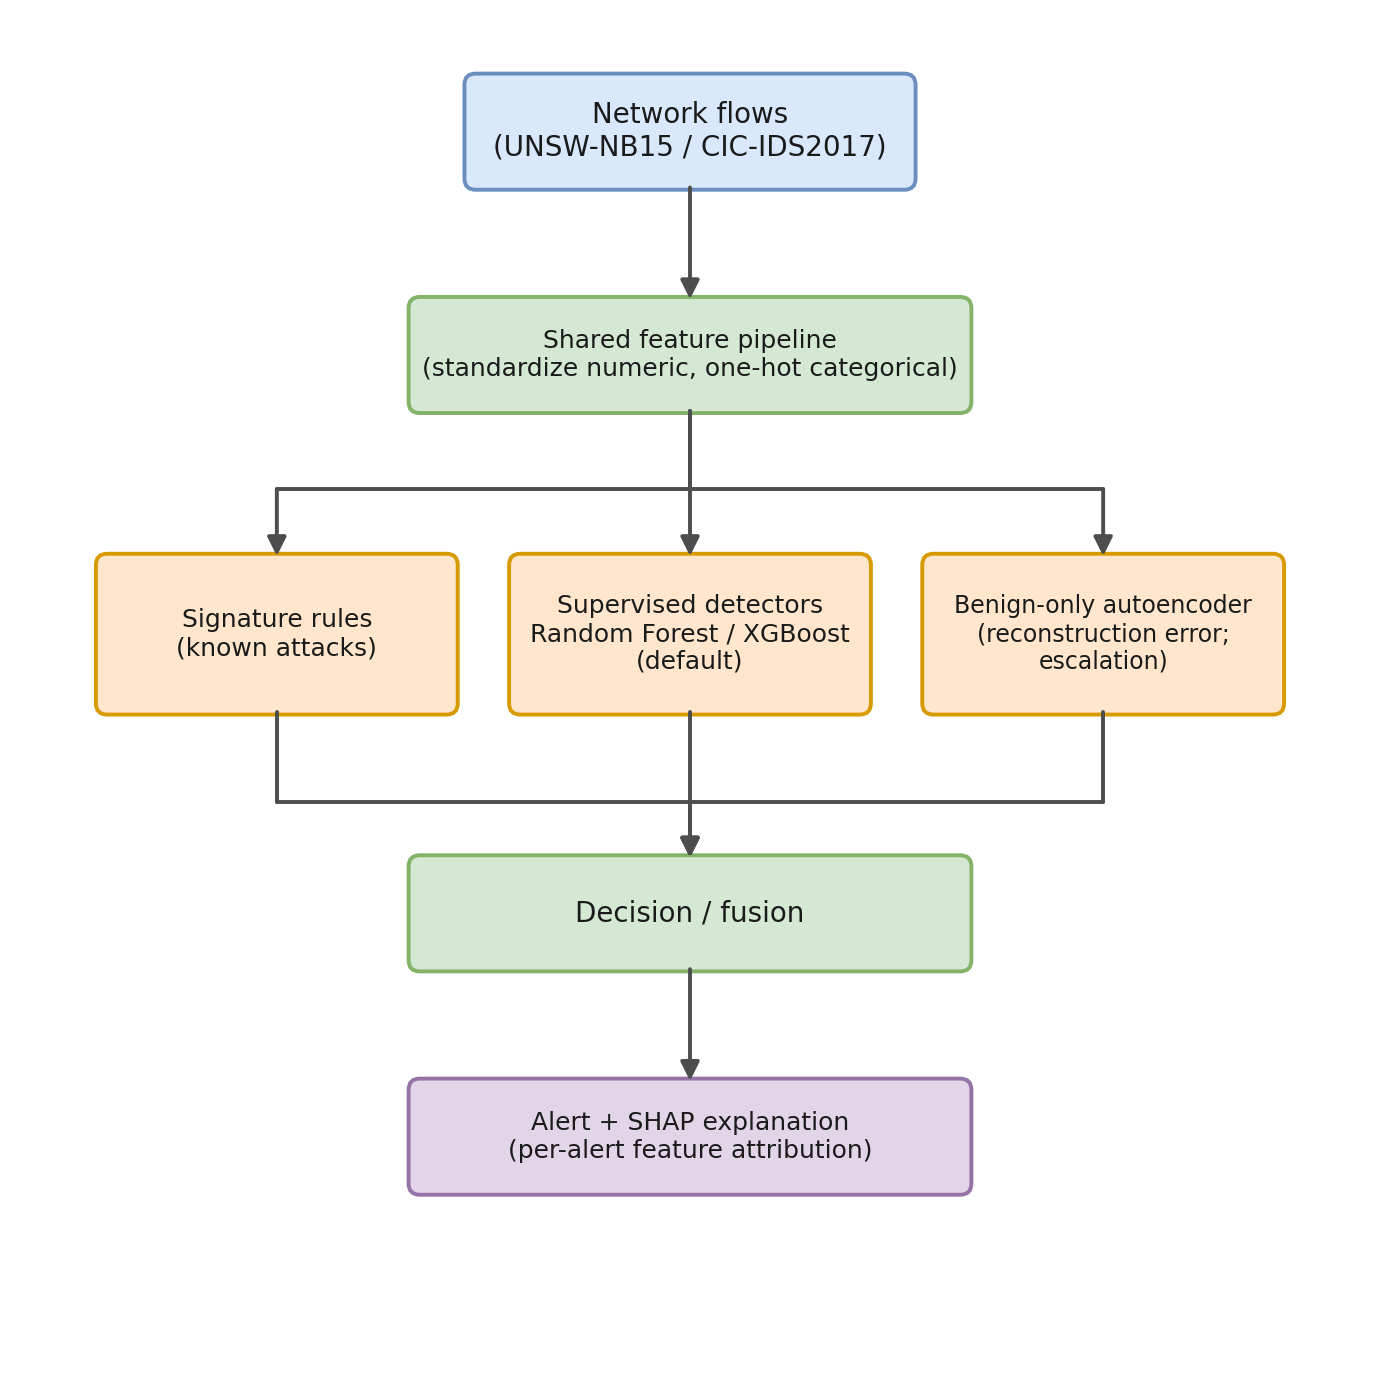
\includegraphics[width=\columnwidth]{fig/architecture.png}
\caption{SHADE pipeline: shared features feed a signature layer, supervised models,
and a benign-only autoencoder; each alert carries a SHAP explanation.}\label{fig:arch}
\end{figure}

\subsection{Leave-One-Family-Out Protocol}
Let the dataset contain benign traffic and attack families
$\mathcal{F}=\{F_1,\dots,F_k\}$. For each held-out family $F_i$ we form a
\emph{known} pool (benign $+$ all families except $F_i$) and a \emph{zero-day} set
(all rows of $F_i$). The known pool is split into stratified train/test partitions.
Supervised models train on the train partition; the autoencoder trains on its benign
rows only. We then build a zero-day test set of benign(test) $\cup\,F_i$ and score it
with each model. Figure~\ref{fig:method} summarizes the full procedure.

\begin{figure}[t]\centering
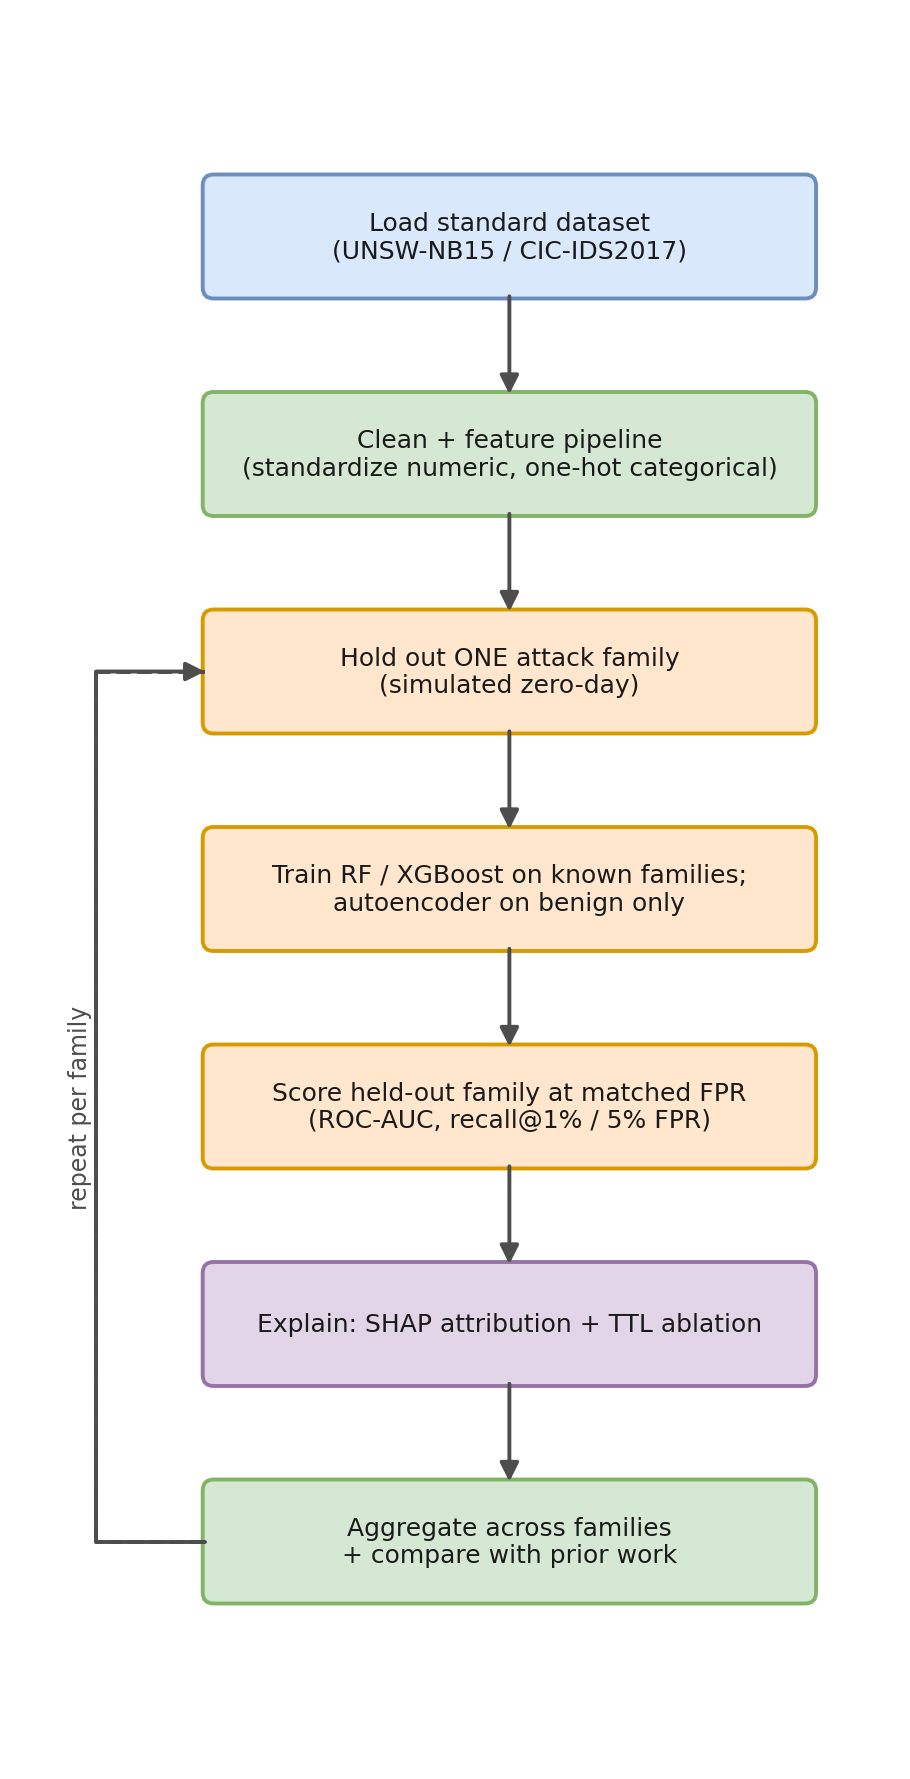
\includegraphics[width=0.78\columnwidth]{fig/methodology.png}
\caption{Leave-one-family-out procedure, repeated for every attack family and then
aggregated and compared against prior work.}\label{fig:method}\end{figure}

\subsection{Models}
Supervised baselines are a Random Forest and XGBoost. The autoencoder $f_\theta$
minimizes reconstruction error on benign traffic,
\begin{equation}
\mathcal{L}(\theta) = \frac{1}{N}\sum_{i=1}^{N}\lVert x_i - f_\theta(x_i)\rVert_2^2 ,
\end{equation}
and its anomaly score at inference is the per-flow reconstruction error.

\subsection{FPR-Matched Comparison}
Because a supervised probability threshold and an autoencoder error threshold are
not directly comparable, we evaluate each model's anomaly score with ROC-AUC over
the zero-day test set, and report recall at a benign false-positive rate fixed to
$1\%$ and $5\%$ (threshold set from the benign-score quantile).

\subsection{Explainability Layer}
We apply SHAP~\cite{shap} to attribute each detection to input flow features: TreeSHAP for the
supervised models and KernelSHAP over the reconstruction-error function for the
autoencoder, computed on flagged alerts to remain tractable.

\section{Experiments and Results}
\subsection{Dataset and Setup}
UNSW-NB15~\cite{unsw_nb15} contributes $257{,}673$ flows ($93{,}000$ benign) across
nine attack families. Numeric features are standardized and categorical features
(\texttt{proto}, \texttt{service}, \texttt{state}) one-hot encoded; the transformer
is fit on training data only. The Random Forest uses $200$ trees and XGBoost $300$
boosting rounds (depth $6$); the autoencoder has encoder dimensions
$64\!\to\!32\!\to\!16$, trained for $50$ epochs (Adam, lr $10^{-3}$, batch $256$).
All experiments run on a commodity desktop CPU; the autoencoder is small enough that GPU
acceleration is not required.

\subsection{Leave-One-Family-Out Generalization}
Table~\ref{tab:loo} reports zero-day detection of each held-out family. Supervised
models generalize strongly to seven of nine families (ROC-AUC $>0.98$). The
benign-only autoencoder, despite using no attack labels, is competitive only on a
subset and is markedly weaker on Shellcode, Reconnaissance, and Worms. \emph{Fuzzers}
is the standout failure for \emph{all} methods: supervised ROC-AUC falls to $0.855$
and recall to $38\%$ at $5\%$ FPR, and the autoencoder ($0.580$ AUC) does not
recover it. Figure~\ref{fig:roc} contrasts the two regimes: for DoS both detectors
work and supervised dominates, whereas for Fuzzers the supervised curve degrades and
the autoencoder collapses toward the diagonal (near-random).

\begin{figure}[t]\centering
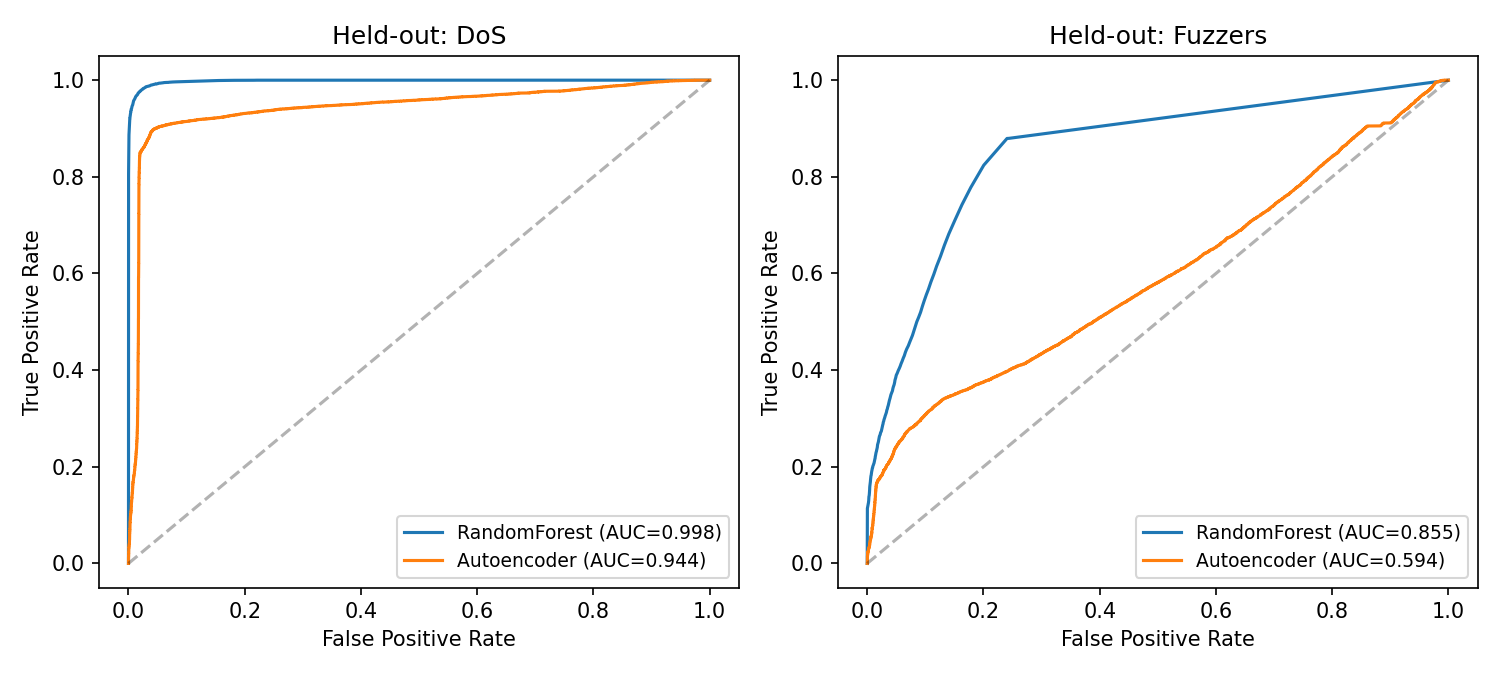
\includegraphics[width=\columnwidth]{fig/roc_zeroday.png}
\caption{Zero-day ROC curves (benign vs.\ held-out family). DoS (left): both
detectors succeed. Fuzzers (right): supervised degrades and the autoencoder is
near-random.}\label{fig:roc}\end{figure}

The single recall-at-FPR number in Table~\ref{tab:loo} hides the autoencoder's
full operating curve. Figure~\ref{fig:thresh} sweeps its decision threshold
$t=\mu+k\sigma$ (where $\mu,\sigma$ are the mean and standard deviation of benign
reconstruction error). For DoS the benign-FPR and recall curves separate, so a
threshold exists that retains high recall at low FPR; for Fuzzers the two curves
track each other and no threshold makes the autoencoder useful---the operating-point
view of its near-random AUC.

\begin{figure}[t]\centering
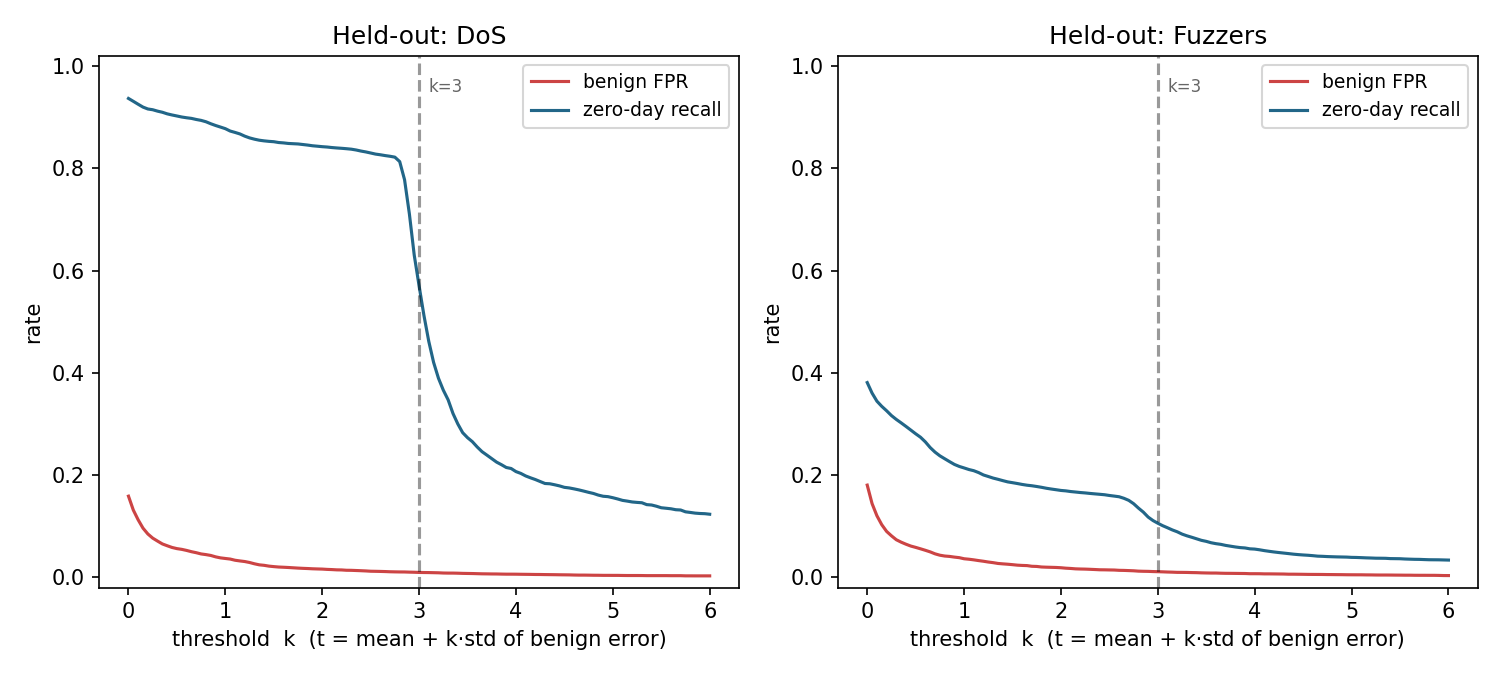
\includegraphics[width=\columnwidth]{fig/ae_threshold_sweep.png}
\caption{Autoencoder threshold sweep: benign FPR and zero-day recall vs.\ the
threshold multiplier $k$ (dashed line: default $k\!=\!3$). DoS (left): the curves
separate, so a usable operating point exists. Fuzzers (right): they track each other,
so recall is never bought without an equal FPR.}\label{fig:thresh}\end{figure}

\begin{table}[t]
\caption{Leave-one-family-out zero-day detection on UNSW-NB15
(sorted by RF ROC-AUC). R@5\% = recall at $5\%$ benign FPR.}
\label{tab:loo}
\centering
\small
\begin{tabular}{lrccccc}
\toprule
Held-out family & $n$ & RF & XGB & AE & RF & AE \\
 & & AUC & AUC & AUC & R@5\% & R@5\% \\
\midrule
Fuzzers        & 24246 & 0.855 & 0.862 & 0.580 & 0.382 & 0.235 \\
Analysis       & 2677  & 0.957 & 0.951 & 0.920 & 0.809 & 0.824 \\
Reconnaissance & 13987 & 0.982 & 0.982 & 0.540 & 0.887 & 0.274 \\
Shellcode      & 1511  & 0.983 & 0.984 & 0.377 & 0.915 & 0.034 \\
Generic        & 58871 & 0.984 & 0.998 & 0.994 & 1.000 & 0.991 \\
Exploits       & 44525 & 0.992 & 0.993 & 0.928 & 0.970 & 0.844 \\
Worms          & 174   & 0.998 & 0.998 & 0.879 & 0.989 & 0.385 \\
DoS            & 16353 & 0.998 & 0.999 & 0.952 & 0.992 & 0.898 \\
Backdoor       & 2329  & 0.999 & 1.000 & 0.946 & 0.999 & 0.912 \\
\bottomrule
\end{tabular}
\end{table}

\subsection{Explainability Results}
To understand \emph{why} generalization varies, we compute TreeSHAP for the
supervised detector on a balanced sample of benign and held-out-family flows.
Across families, a single feature---\texttt{sttl} (source time-to-live)---dominates
the attributions (mean$|$SHAP$|$ $\approx 4.5$--$4.7$, several times any other
feature). Low \texttt{sttl} values push strongly toward the benign class, so the
model appears to learn a TTL-based separator that transfers across attack families.
However, this attribution is misleading on its own: ablating \texttt{sttl}---or the
entire TTL group (\texttt{sttl}, \texttt{dttl}, \texttt{ct\_state\_ttl})---leaves
performance essentially unchanged (Section~\ref{sec:ablation}). The TTL signal is
\emph{redundantly encoded} across correlated features, so high SHAP attribution does
not imply necessity. The practical lesson is twofold: cross-family generalization on
UNSW-NB15 is robust rather than a fragile single-feature shortcut, and feature
importance in correlated NIDS feature spaces must be validated by ablation, not read
from attribution alone.

For DoS (Fig.~\ref{fig:shap-dos}), attributions concentrate on \texttt{sttl} and
\texttt{ct\_state\_ttl}, giving a clean separator and high recall. For Fuzzers
(Fig.~\ref{fig:shap-fuzzers}), importance is more diffuse---\texttt{sttl} still
leads but \texttt{ct\_dst\_src\_ltm}, \texttt{sbytes}, and \texttt{smean} contribute
comparably---indicating no single reliable separator and explaining the degraded
generalization (ROC-AUC $0.855$).

\begin{figure}[t]\centering
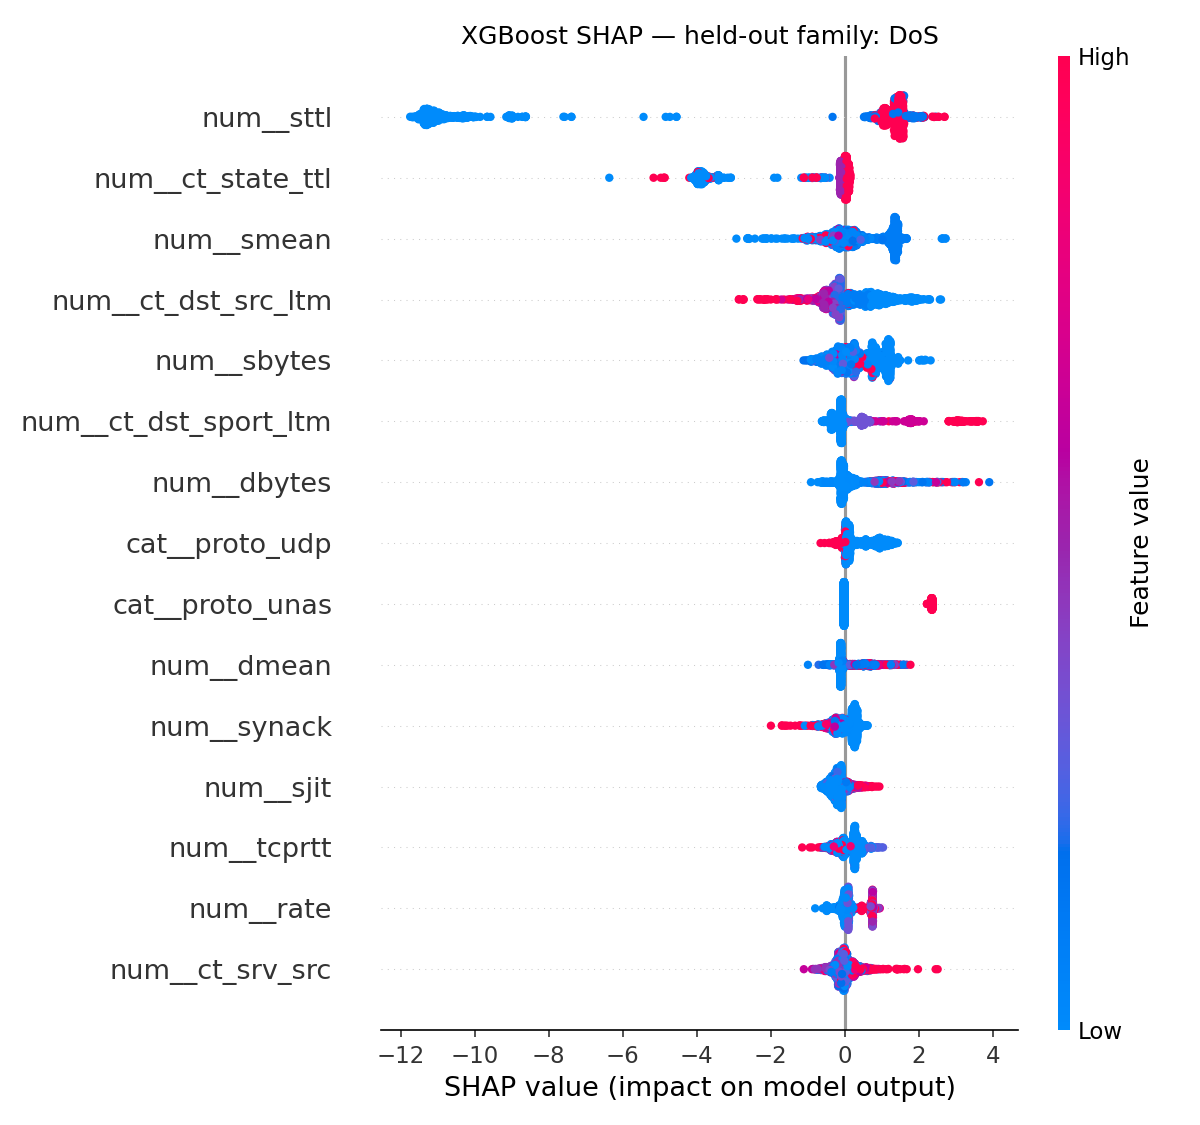
\includegraphics[width=\columnwidth]{fig/shap_rf_holdout_DoS.png}
\caption{SHAP attributions, held-out DoS: a clean \texttt{sttl}/\texttt{ct\_state\_ttl}
separator.}\label{fig:shap-dos}\end{figure}

\begin{figure}[t]\centering
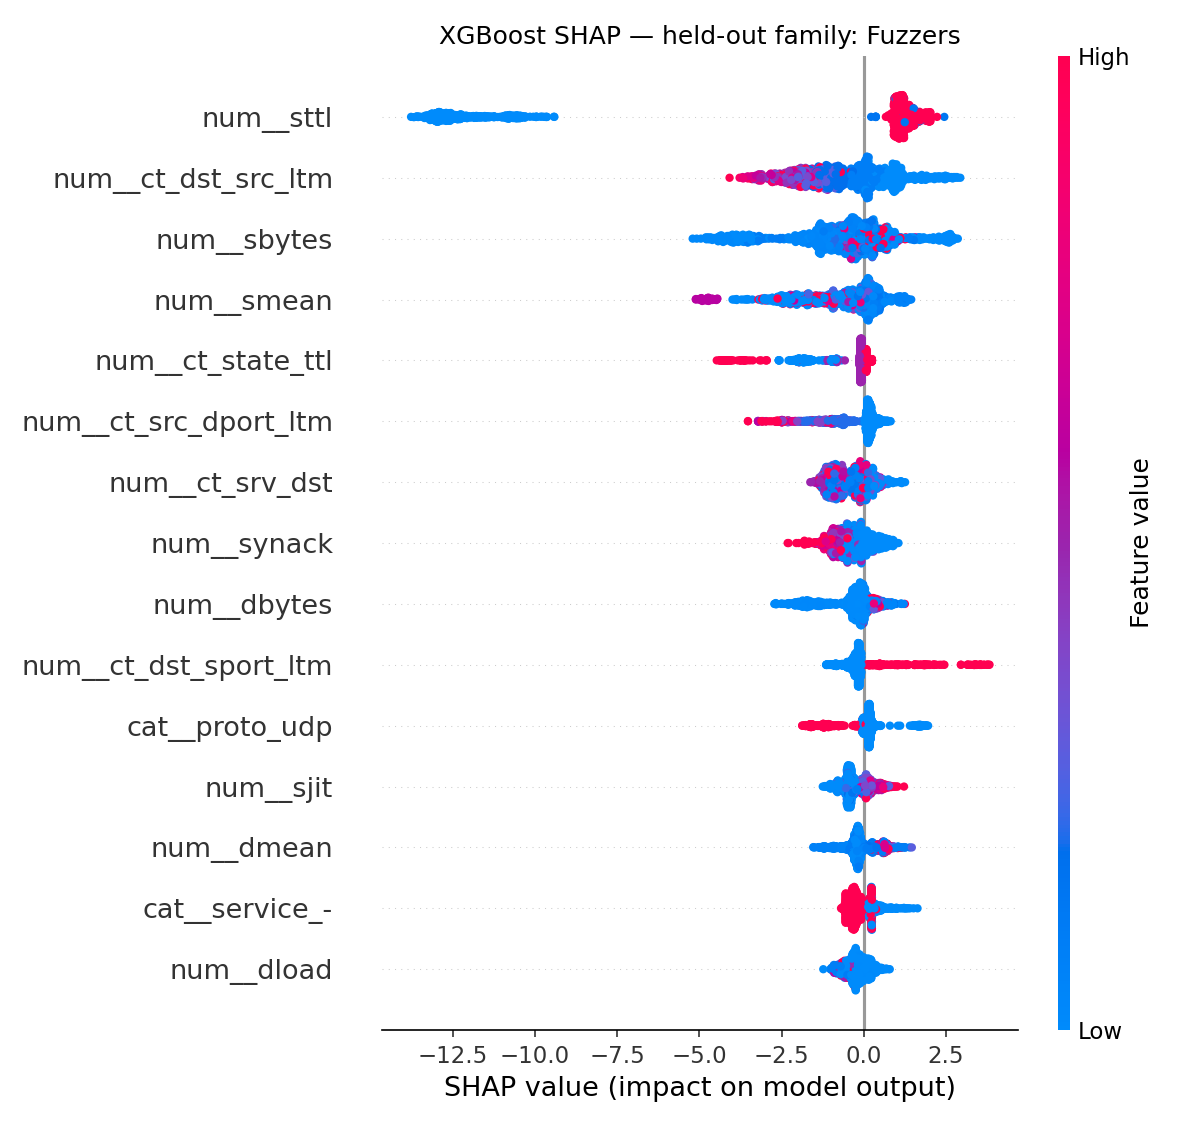
\includegraphics[width=\columnwidth]{fig/shap_rf_holdout_Fuzzers.png}
\caption{SHAP attributions, held-out Fuzzers: importance is diffuse, so no single
feature cleanly separates the unseen family.}\label{fig:shap-fuzzers}\end{figure}

\subsection{Feature Ablation: Is It Really the TTL Shortcut?}\label{sec:ablation}
Because SHAP attributes most of the decision to \texttt{sttl}, we test whether
generalization actually \emph{depends} on it by re-running the full leave-one-family-out
study with TTL features removed. Table~\ref{tab:ablation} shows that dropping
\texttt{sttl} alone, or the whole TTL group, changes Random Forest ROC-AUC by at most
$0.003$ on any family. Generalization is therefore not contingent on the TTL artifact;
the discriminative signal is redundantly carried by correlated features. This is a
cautionary result for explainable IDS: a feature can dominate SHAP attributions yet be
entirely dispensable.

\begin{table}[t]
\caption{Random Forest zero-day ROC-AUC is robust to removing TTL features.}
\label{tab:ablation}
\centering
\small
\begin{tabular}{lccc}
\toprule
Held-out family & All features & $-$\texttt{sttl} & $-$TTL group \\
\midrule
Fuzzers        & 0.855 & 0.855 & 0.852 \\
Analysis       & 0.957 & 0.957 & 0.957 \\
Reconnaissance & 0.982 & 0.982 & 0.982 \\
Shellcode      & 0.983 & 0.983 & 0.982 \\
Generic        & 0.984 & 0.983 & 0.981 \\
Exploits       & 0.992 & 0.992 & 0.991 \\
Worms          & 0.998 & 0.997 & 0.997 \\
DoS            & 0.998 & 0.998 & 0.998 \\
Backdoor       & 0.999 & 0.999 & 0.999 \\
\bottomrule
\end{tabular}
\end{table}

\subsection{Cross-Dataset Validation (CIC-IDS2017)}\label{sec:crossdataset}
To test whether our findings are an artifact of UNSW-NB15, we repeat the
leave-one-family-out protocol on CIC-IDS2017~\cite{cicids2017}, an independent dataset
with a different feature schema (52 CICFlowMeter flow statistics). We use a cleaned, class-capped
subsample of $203{,}241$ flows ($100{,}000$ benign) spanning six attack families.
Table~\ref{tab:cicids} shows the same qualitative pattern as UNSW-NB15: supervised
models generalize strongly to most unseen families (DoS, DDoS, Brute Force, Web
Attacks; ROC-AUC $>0.97$), the label-free autoencoder rarely helps, and there are
clear supervised blind spots---here \emph{Bots} (ROC-AUC $0.639$) and \emph{Port
Scanning} ($0.779$). Crucially, on these blind-spot families the autoencoder is no
better (Bots $0.662$, Port Scanning $0.778$), reproducing the central UNSW-NB15
result that anomaly detection is not a reliable safety net for the families
supervised models miss. The pattern thus holds across two datasets.

\begin{table}[t]
\caption{Leave-one-family-out on CIC-IDS2017 (sorted by RF ROC-AUC). The pattern
matches UNSW-NB15: strong supervised generalization with blind spots (Bots, Port
Scanning) where the autoencoder also fails.}
\label{tab:cicids}
\centering
\small
\begin{tabular}{lccccc}
\toprule
Held-out family & RF & XGB & AE & RF & AE \\
 & AUC & AUC & AUC & R@5\% & R@5\% \\
\midrule
Bots          & 0.639 & 0.698 & 0.662 & 0.084 & 0.024 \\
Port Scanning & 0.779 & 0.787 & 0.778 & 0.140 & 0.025 \\
Brute Force   & 0.974 & 0.976 & 0.704 & 0.997 & 0.000 \\
DDoS          & 0.989 & 0.961 & 0.915 & 1.000 & 0.635 \\
DoS           & 0.991 & 0.997 & 0.960 & 0.975 & 0.862 \\
Web Attacks   & 0.996 & 0.999 & 0.654 & 1.000 & 0.044 \\
\bottomrule
\end{tabular}
\end{table}

\subsection{Comparison with Prior Work}\label{sec:priorwork}
Table~\ref{tab:priorwork} places our results next to representative UNSW-NB15 studies.
Random-split evaluations report near-perfect accuracy (e.g.\ Random Forest at
$\approx 98.7\%$~\cite{kasongo_unsw}), but they test on the \emph{same} attack families
seen in training and therefore do not measure zero-day generalization. Studies that do
hold attacks out report lower, more honest numbers: Lotfi and Lotfi~\cite{lotfi_zeroday}
hold out four rare families \emph{jointly} and obtain Random Forest zero-day ROC-AUC
$0.913$ (rising to $0.968$ only with SMOTE oversampling), and Sarhan
et~al.~\cite{sarhan_zeroshot} report sharp drops for certain attack groups under a
zero-shot protocol. Crucially, both evaluate supervised models in isolation: neither
compares, at a matched false-positive rate, against a label-free anomaly detector on the
unseen families.

Our study differs on three axes. First, granularity: holding out each family
\emph{individually} rather than as a pooled rare-attack set localizes the blind spot to
\emph{Fuzzers} (RF AUC $0.855$), which a combined holdout of rare families
(all of which we detect at AUC $\geq 0.957$) would mask. Second, the FPR-matched
supervised-vs-autoencoder comparison shows the anomaly detector does not recover these
blind spots. Third, SHAP plus ablation explains \emph{why} generalization holds or fails.
Against the standard label-free zero-day technique (the autoencoder), our supervised-first
detector improves zero-day ROC-AUC on every UNSW-NB15 family (e.g.\ Reconnaissance
$0.540\!\to\!0.982$, Shellcode $0.377\!\to\!0.983$; Table~\ref{tab:loo}).

\begin{table}[t]
\caption{Positioning against representative UNSW-NB15 prior work. ID = in-distribution
(random split); LOO = leave-one-family-out. ``AE cmp.''\ = matched comparison against a
label-free autoencoder.}
\label{tab:priorwork}
\centering
\small
\begin{tabular}{llll}
\toprule
Study & Protocol & RF result & AE cmp. \\
\midrule
Kasongo \& Sun~\cite{kasongo_unsw}   & ID random split      & $0.987$ acc          & no \\
Sarhan et~al.~\cite{sarhan_zeroshot} & zero-shot, per-group & drops on some groups & no \\
Lotfi \& Lotfi~\cite{lotfi_zeroday}  & rare families pooled & $0.913$ AUC          & no \\
\textbf{SHADE (ours)}                & per-family LOO       & $0.855$--$0.999$ AUC & yes \\
\bottomrule
\end{tabular}
\end{table}

\section{Discussion}
The results argue against deploying an unsupervised anomaly detector as a blanket
zero-day safeguard. Across \emph{both} datasets, it is dominated by supervised
generalization on most families and---critically---fails on the very families the
supervised models miss (Fuzzers on UNSW-NB15; Bots and Port Scanning on
CIC-IDS2017), so it does not function as a safety net where one is most needed. Its
genuine advantage is operational: it needs no attack labels, making it useful in
cold-start or low-label settings rather than as a universal detector. The actionable
design is therefore a hybrid that defaults to an explainable supervised model and
escalates to anomaly detection only for families exhibiting weak supervised
generalization. That the same pattern recurs on two datasets with different feature
schemas suggests it reflects a property of binary NIDS generalization rather than a
quirk of one benchmark.

\noindent\textbf{Limitations.} We adopt a binary attack/benign framing; a multi-class
formulation that explicitly rejects ``unknown'' families is left to future work. Both
datasets are benchmark captures rather than live enterprise traffic, and our
CIC-IDS2017 evaluation uses a class-capped subsample, so absolute numbers may shift at
full scale; the qualitative cross-dataset agreement is the robust finding. Finally,
the blind-spot families (Fuzzers, Bots, Port Scanning) are internally heterogeneous,
which likely contributes to their poor separability and merits dedicated study.

\section{Conclusion}
We mapped where supervised NIDS generalize to unseen attack families on
\emph{two} datasets (UNSW-NB15 and CIC-IDS2017), showing strong generalization for
most families with consistent blind spots (Fuzzers; Bots and Port Scanning) where the
label-free autoencoder also fails, and used SHAP plus feature ablation to explain the
pattern. \textsc{Shade} operationalizes this as an explainable supervised-first
hybrid. Future work: multi-class ``unknown'' rejection for the blind-spot families,
evaluation on live operational traffic, and adversarial robustness
\cite{shap_fingerprint}.

\bibliographystyle{IEEEtran}
\bibliography{references}

\end{document}
